\documentclass[11pt,a4paper]{article}
\usepackage[T1]{fontenc}
\usepackage[utf8]{inputenc}
\usepackage[french]{babel}
\usepackage{lmodern}
\usepackage{amsmath,amssymb}
\usepackage[margin=2.25cm]{geometry}
\usepackage{booktabs,tabularx}
\usepackage{graphicx}
\usepackage{float}
\usepackage{enumitem}
\usepackage{xcolor}
\usepackage{microtype}
\usepackage{hyperref}

\hypersetup{colorlinks=true,linkcolor=blue!45!black,urlcolor=blue!45!black}
\setlist{nosep}
\newcommand{\E}{\mathbb E}
\newcommand{\Pp}{\mathbb P}

\title{Répartitions empiriques dans la dyade de crédit M4.2\\
\large Prêt à égalisation arithmétique et variation du capital initial $k_2$}
\author{Complément empirique à l'étude analytique du prêt unique}
\date{29 juillet 2026}

\begin{document}
\maketitle

\begin{abstract}
Ce rapport estime par Monte-Carlo les lois asymptotiques et arrêtées de la
dyade définie dans l'étude analytique. Une entité de capital $k_1=100$
accorde une unique dette perpétuelle à une entité de capital initial
$k_2<k_1$. Le principal est exclusivement celui de l'égalisation
arithmétique, $q=(k_1-k_2)/2$ ; la règle géométrique n'est pas étudiée ici.
La campagne croise six valeurs de $k_2$ et huit taux, à raison de
$100\,000$ trajectoires par condition. Elle estime la loi du temps de
défaut $T_B$, les capitaux arrêtés $(L_{T_B},B_{T_B}^{\dagger})$ et la loi
stationnaire autarcique de la prêteuse après disparition du contrat. Les
résultats confirment que $T_B$ augmente fortement avec $k_2$ et décroît
avec le taux. À $r=0{,}1$, sa médiane passe de 2 pas pour $k_2=5$ à 110
pas pour $k_2=60$. Les décès sont presque tous des insolvabilités avec
service intégral, et non des défauts de liquidité.
\end{abstract}

\tableofcontents

\section{Objet et variables aléatoires}

Les notations sont celles du rapport analytique. Juste avant l'unique prêt,
\[
k_1=100>k_2>0.
\]
La règle arithmétique fixe
\begin{equation}
q=\frac{k_1-k_2}{2},\qquad
L_0=B_0=\frac{k_1+k_2}{2},\qquad c=rq.
\label{eq:initial}
\end{equation}
La production est $K^\gamma$, la dépréciation est $\delta$, et les
multiplicateurs de choc sont exactement ceux de M4.2 :
\begin{equation}
X_{i,t}=e^{\xi_{i,t}},\qquad
\xi_{i,t}\sim\mathcal N(-\sigma^2/2,\sigma^2),
\qquad \E X_{i,t}=1.
\label{eq:shock}
\end{equation}

Les variables empiriques sont :
\begin{itemize}
\item $T_B\in\mathbb N^*\cup\{+\infty\}$, temps de mort de
l'emprunteuse ;
\item $B_{T_B}^{\dagger}\in[0,q)$, capital résiduel juste avant sa
destruction ;
\item $L_{T_B}>0$, capital de la prêteuse au même pas, après paiement et
dépréciation ;
\item la cause du décès : défaut de liquidité si les ressources avant
service sont sous $rq$, insolvabilité sinon ;
\item $L_\infty$ au sens de la loi stationnaire autarcique
$\pi_{\gamma,\delta,\sigma}$.
\end{itemize}

La prêteuse ne meurt jamais dans cette expérience, donc
$T_L=+\infty$ avec probabilité un et sa « répartition empirique » est
dégénérée. De même, $B_\infty$ est le point cimetière presque sûrement.
La seule loi réelle asymptotique non dégénérée est celle de $L_\infty$.

\section{Plan de Monte-Carlo}

\subsection{Grille principale}

La configuration centrale est
\begin{equation}
(\gamma,\delta,\sigma)=(1/2,0{,}05,0{,}25),
\qquad k_1=100.
\label{eq:baseline}
\end{equation}
La grille croisée est
\begin{align}
k_2&\in\{5,10,25,40,50,60\},\\
r&\in\{0;0{,}025;0{,}05;0{,}07071;0{,}1;0{,}25;0{,}5;1\}.
\end{align}
La valeur $0{,}07071$ est le taux géométrique marginal instantané de M4.2
aux capitaux pré-prêt $(100,25)$ pour $\gamma=1/2$ ; elle sert uniquement
de repère de taux, sans réintroduire la règle géométrique de principal.

Chaque condition contient $N=100\,000$ trajectoires indépendantes, avec
un horizon $H=20\,000$. Les 48 conditions de la grille principale sont
toutes intégralement absorbées avant $H$. Les valeurs $k_2=75$ et 90,
sondées pendant la conception, ont été écartées : à faible taux, leur
défaut est trop rare pour estimer une loi non censurée par Monte-Carlo
brut dans un temps raisonnable.

\subsection{Sensibilités et loi stationnaire}

À $(k_2,r)=(25,0{,}1)$, on fait varier séparément
\[
\gamma\in\{1/3,1/2,2/3\},\quad
\delta\in\{0{,}02;0{,}05;0{,}10\},\quad
\sigma\in\{0{,}10;0{,}25;0{,}40\}.
\]
La loi autarcique est approchée par $40\,000$ particules pendant
$2\,500$ pas. Une moitié part de $0{,}01K_{\rm aut}$ et l'autre de
$100K_{\rm aut}$, afin de contrôler l'oubli de l'état initial.

\subsection{Parallélisation et précision}

La campagne est exécutée sur 8 processus. Chaque condition d'arrêt est
découpée en 16 sous-échantillons indépendants, y compris le contrôle
couplé. Les graines sont déterminées par une fonction stable du nom de la
condition et du numéro de sous-échantillon. La campagne complète dure
1 min 14 s sur la machine de calcul et utilise au plus 516 Mio de mémoire
pour le processus principal.

Pour $N=100\,000$, la borne uniforme de Dvoretzky--Kiefer--Wolfowitz à
95\,\% vaut
\begin{equation}
\varepsilon_N=\sqrt{\frac{\log(40)}{2N}}\simeq0{,}00430.
\label{eq:dkw}
\end{equation}
L'écart maximal observé entre la probabilité analytique et la fréquence de
$T_B=1$ est $0{,}00210$, inférieur à cette borne.

\section{Effet du capital initial \texorpdfstring{$k_2$}{k2}}

Le tableau~\ref{tab:k2} donne les répartitions à $r=0{,}1$. Augmenter
$k_2$ produit simultanément
\[
q=\frac{100-k_2}{2}\downarrow,
\qquad B_0=\frac{100+k_2}{2}\uparrow.
\]
Les deux effets retardent le franchissement de la contrainte $B<q$.

\begin{table}[H]
\centering
\resizebox{\textwidth}{!}{\input{resultats/table_k2.tex}}
\caption{Quantiles empiriques selon $k_2$, pour $r=0{,}1$. La colonne
liquidité donne la part des décès dus à un service incomplet.}
\label{tab:k2}
\end{table}

La médiane de $T_B$ passe de 2 à 110 pas entre $k_2=5$ et $k_2=60$ ; le
quantile 99\,\% passe de 91 à 824. La dispersion croît donc avec la durée
typique. Les fonctions de survie de la figure~\ref{fig:survival} ne sont
pas de simples translations : leurs queues s'allongent lorsque le
principal diminue.

\begin{figure}[H]
\centering
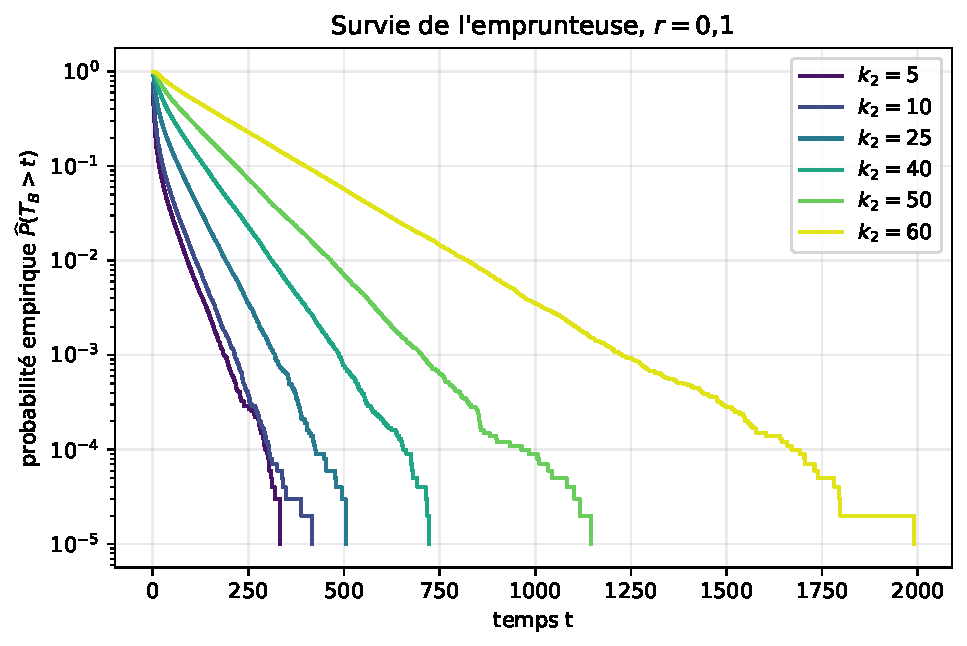
\includegraphics[width=.78\textwidth]{figures/survie_baseline.pdf}
\caption{Fonctions de survie empiriques de $T_B$ à $r=0{,}1$ ; axe
vertical logarithmique.}
\label{fig:survival}
\end{figure}

Le capital terminal relatif $B_{T_B}^{\dagger}/q$ est concentré près de
un : sa médiane varie de $0{,}869$ à $0{,}900$. L'emprunteuse paie donc le
plus souvent la rente complète puis devient insolvable parce que son
capital déprécié tombe juste sous le principal nominal. Cela explique
l'absence de défaut de liquidité à trois décimales pour $r=0{,}1$.

\begin{figure}[H]
\centering
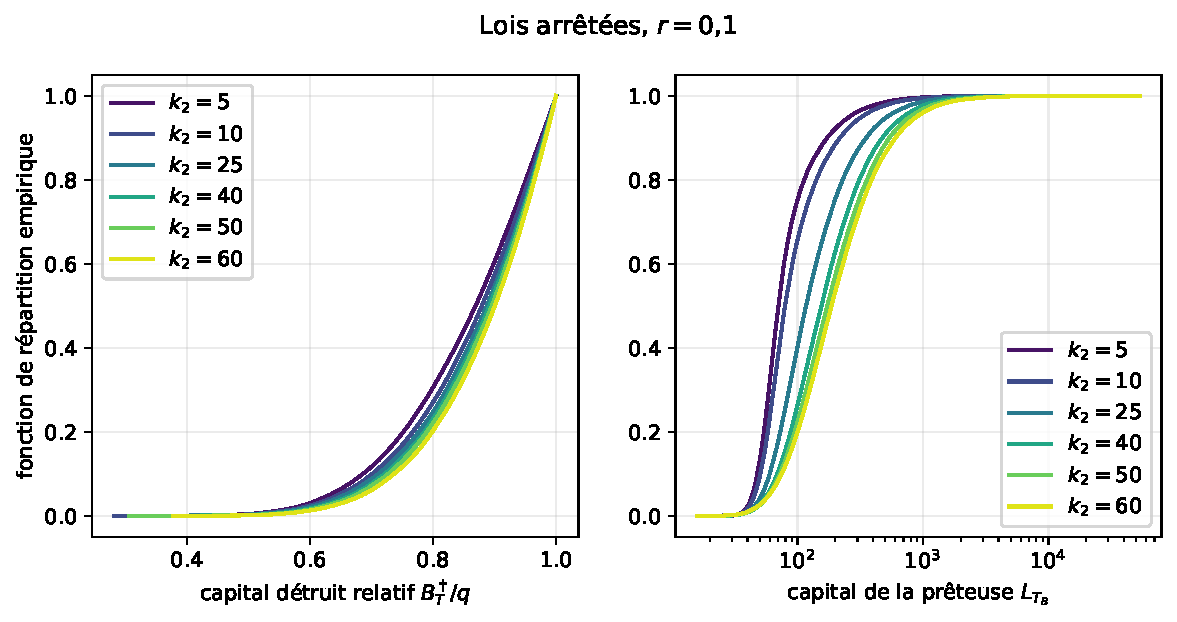
\includegraphics[width=.96\textwidth]{figures/lois_capitaux_arretes.pdf}
\caption{Fonctions de répartition de $B_{T_B}^{\dagger}/q$ et de
$L_{T_B}$ à $r=0{,}1$.}
\label{fig:stopped-capitals}
\end{figure}

La médiane de $L_{T_B}$ croît de 70,3 à 186,7 avec $k_2$. Cette croissance
ne mesure pas seulement la rente : lorsque $k_2$ augmente, la prêteuse
part elle-même avec un capital égalisé plus grand et dispose de beaucoup
plus de temps avant le défaut.

\section{Interaction entre \texorpdfstring{$k_2$}{k2} et le taux}

\begin{figure}[H]
\centering
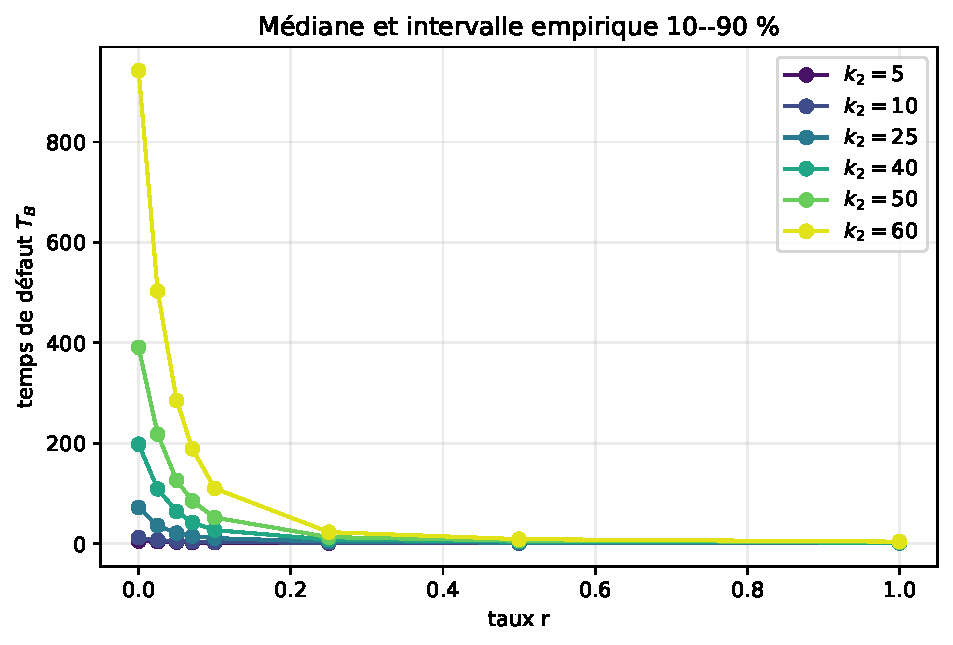
\includegraphics[width=.78\textwidth]{figures/temps_defaut_selon_taux.pdf}
\caption{Médiane de $T_B$ selon le taux, pour les six valeurs de $k_2$.}
\label{fig:rate-time}
\end{figure}

Le taux raccourcit la durée de vie pour tout $k_2$, conformément à l'ordre
trajectoriel analytique. À $k_2=25$, la médiane passe de 72 pas à taux nul
à un pas pour $r=1$.

\begin{table}[H]
\centering
\input{resultats/table_taux.tex}
\caption{Effet du taux à $k_2=25$.}
\label{tab:rate}
\end{table}

L'interaction est très forte. À taux nul, la médiane est multipliée par
environ 188 entre $k_2=5$ et 60 ; à $r=1$, elle ne passe que de 1 à 4.
La rente élevée domine donc progressivement l'avantage initial conféré par
un petit principal.

\begin{figure}[H]
\centering
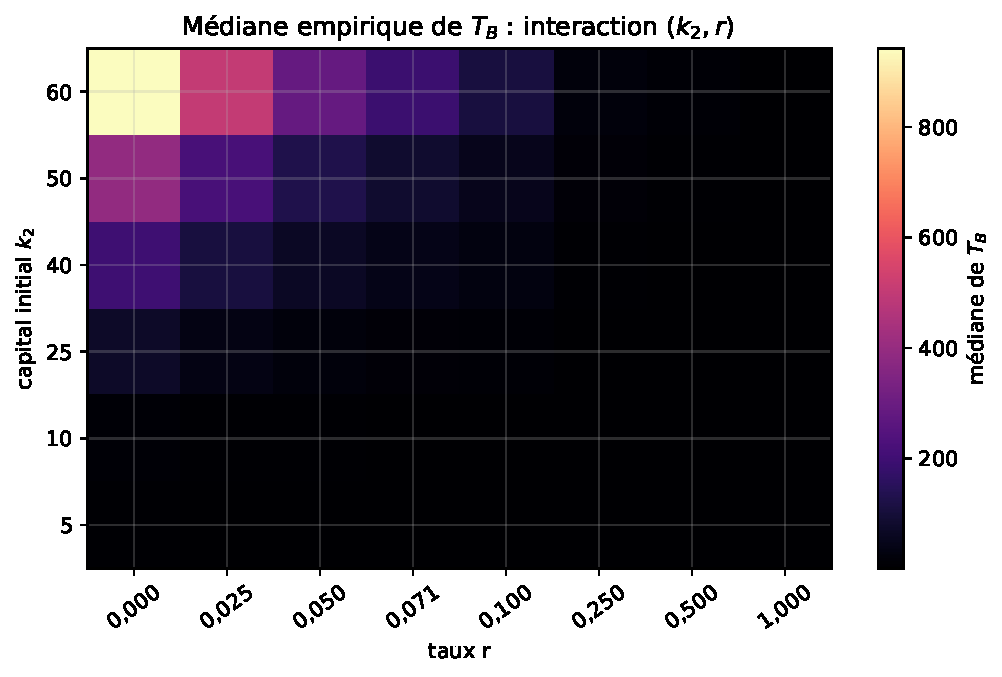
\includegraphics[width=.80\textwidth]{figures/carte_mediane_k2_taux.pdf}
\caption{Carte de la médiane de $T_B$ sur la grille $(k_2,r)$.}
\label{fig:heatmap}
\end{figure}

Les défauts de liquidité restent pratiquement absents jusqu'à $r=0{,}5$.
À $r=1$, ils représentent de 4,1\,\% à 19,9\,\% des décès suivant
$k_2$ ; l'insolvabilité avec paiement complet demeure majoritaire.

\begin{figure}[H]
\centering
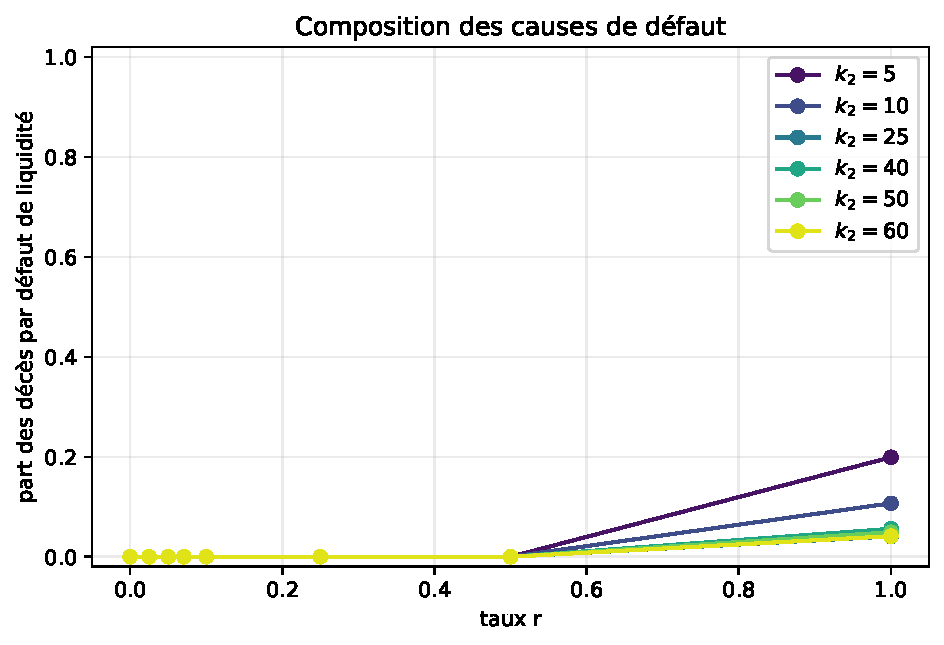
\includegraphics[width=.78\textwidth]{figures/causes_selon_taux.pdf}
\caption{Part des défauts de liquidité selon $(k_2,r)$.}
\label{fig:causes}
\end{figure}

La médiane de $L_{T_B}$ n'est pas monotone en $r$. Pour $k_2=25$, elle
vaut 115,1 à $r=0$, culmine à 120,0 vers $r=0{,}05$, puis tombe à 105,4
pour $r=0{,}5$ avant de remonter légèrement à 108,0 pour $r=1$. Cette
statistique ne définit pas un taux optimal : elle compare des temps
d'arrêt différents et ne tient compte ni d'une actualisation ni de
l'utilité intertemporelle.

\section{Sensibilités en
\texorpdfstring{$\gamma$, $\delta$ et $\sigma$}{gamma, delta et sigma}}

\begin{table}[H]
\centering
\input{resultats/table_sensibilites.tex}
\caption{Sensibilités à $(k_2,r)=(25,0{,}1)$. Pour $\gamma=2/3$, 46,98\,\%
des trajectoires sont censurées à 20 000 ; le quantile 90\,\% est donc
seulement borné inférieurement.}
\label{tab:sensitivity}
\end{table}

Dans cette échelle non normalisée, augmenter $\gamma$ augmente très
fortement la durée de vie : la médiane vaut 5, 11 puis 17 903. Ce résultat
combine la courbure et le déplacement considérable de l'échelle
autarcique ; il ne doit pas être interprété comme un effet pur de
concavité. Pour $\gamma=2/3$, la fonction de répartition empirique atteint
seulement $0{,}53022$ à l'horizon : la médiane est identifiable mais pas
les quantiles 90\,\% et 99\,\%.

Une dépréciation plus forte raccourcit sans ambiguïté la survie : les
médianes sont 21, 11 et 6. Sur la grille choisie, une volatilité plus
forte la raccourcit aussi fortement, de 273 pas à $\sigma=0{,}1$ à 5 pas
à $\sigma=0{,}4$. Ce dernier classement est empirique et local à la grille ;
le risque instantané n'est pas monotone en $\sigma$ pour tous les états.

\begin{figure}[H]
\centering
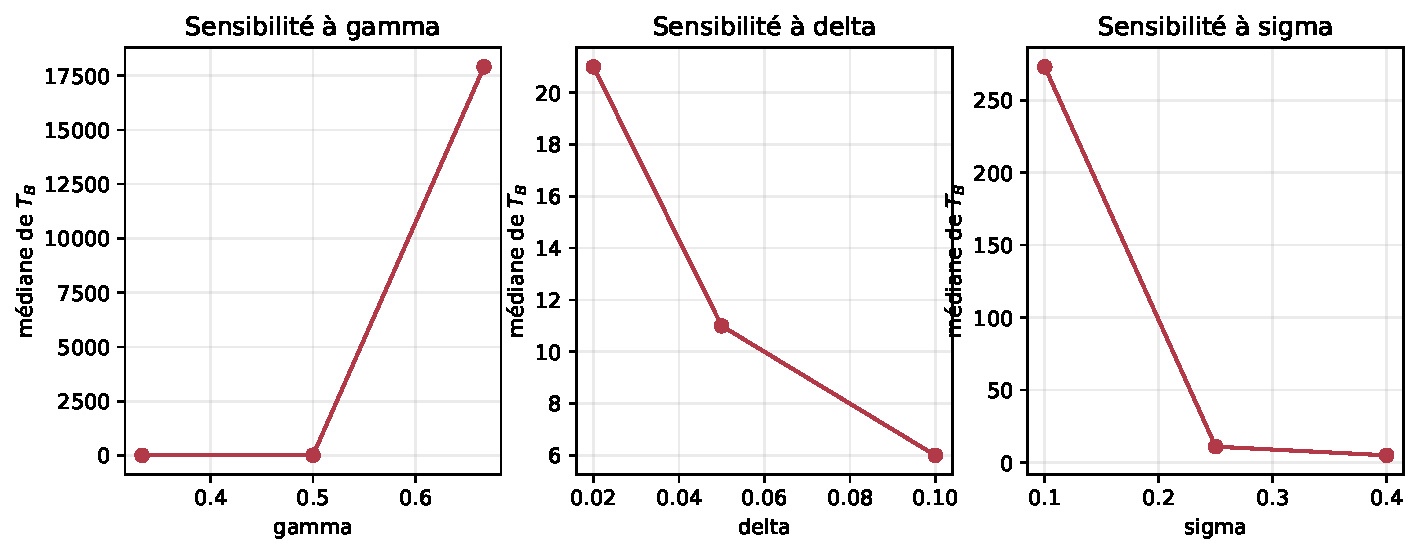
\includegraphics[width=.96\textwidth]{figures/sensibilites_temps_defaut.pdf}
\caption{Médiane empirique de $T_B$ dans les trois analyses de
sensibilité.}
\label{fig:sensitivity}
\end{figure}

\section{Loi stationnaire asymptotique de la prêteuse}

Après la mort de l'emprunteuse, le contrat disparaît et la prêteuse suit
\[
L_{t+1}=(1-\delta)
\left[L_te^{\xi_{t+1}}+(L_te^{\xi_{t+1}})^\gamma\right].
\]
Sa loi limite ne dépend plus de $k_2$, de $q$ ni de $r$. Sous la
configuration centrale, sa médiane vaut 157,6, sa moyenne 275,0, son
quantile 90\,\% 550,2 et son quantile 99\,\% 1 922,1. Le point fixe
déterministe $K_{\rm aut}=361$ n'est donc ni la médiane ni la moyenne de
la loi stochastique.

\begin{figure}[H]
\centering
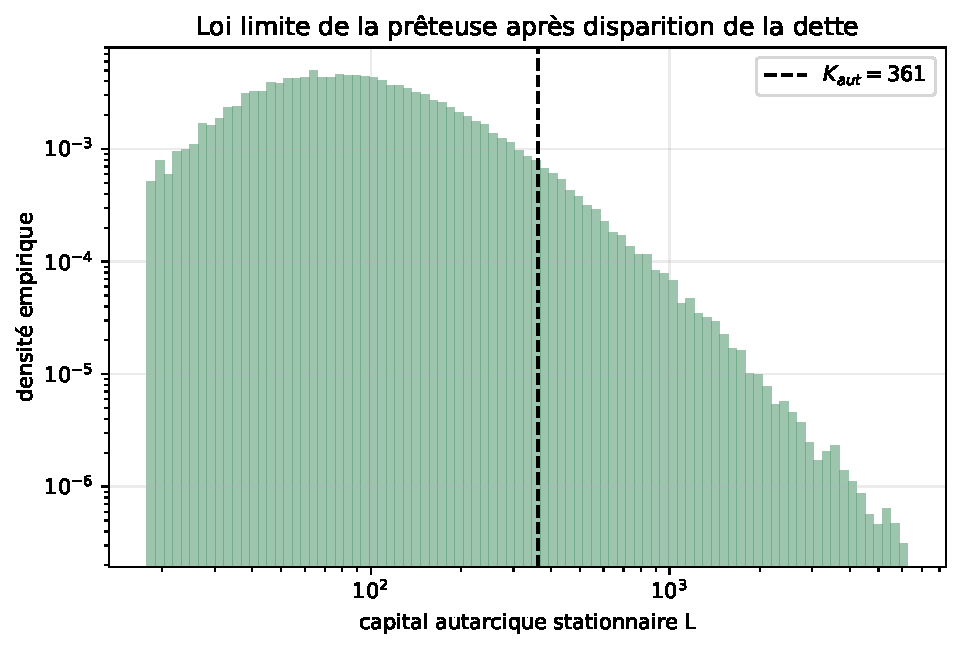
\includegraphics[width=.76\textwidth]{figures/loi_stationnaire_preteuse.pdf}
\caption{Densité empirique de la loi stationnaire centrale ; les deux axes
sont logarithmiques.}
\label{fig:stationary}
\end{figure}

\begin{table}[H]
\centering
\resizebox{\textwidth}{!}{\input{resultats/table_stationnaire.tex}}
\caption{Quantiles des lois stationnaires. « KS init. » compare, au temps
final, les particules parties des deux conditions initiales extrêmes. Le
résidu moment teste l'identité stationnaire du rapport analytique.}
\label{tab:stationary}
\end{table}

Les distances KS entre les deux groupes initiaux restent entre 0,0053 et
0,0117, ce qui indique un oubli satisfaisant des conditions initiales. Le
résidu relatif de l'identité de moment est 0,0046 au centre. Il monte à
0,0429 pour $\delta=0{,}02$, régime à queue très lourde où la moyenne est
beaucoup moins stable que les quantiles ; les quantiles doivent y être
préférés.

\section{Contrôles et limites}

\begin{enumerate}
\item Les 48 distributions de la grille $(k_2,r)$ sont sans censure à
$H=20\,000$.
\item Sur 100 000 vecteurs couplés par la même suite de chocs, aucune
violation de
\[
T_B(5)\leq T_B(10)\leq\cdots\leq T_B(60)
\]
n'est observée ; les deux extrêmes sont strictement ordonnés dans les
100 000 cas.
\item L'erreur maximale sur la probabilité analytique de décès au premier
pas est 0,00210, compatible avec la précision uniforme
\eqref{eq:dkw}.
\item Le seul résultat censuré est la sensibilité $\gamma=2/3$. Les
quantiles non identifiables sont notés $>20\,000$ et non calculés sur les
seuls décès observés.
\item La campagne reste conditionnelle à $k_1=100$ et à la règle
arithmétique. Elle ne compare aucune autre institution de principal.
\end{enumerate}

\section{Conclusion}

Pour l'égalisation arithmétique, $k_2$ est un levier majeur de la loi de
défaut parce qu'il agit deux fois : il augmente le capital post-prêt de
l'emprunteuse et réduit le principal nominal qui borne sa valeur nette.
La totalité de la grille confirme l'ordre prévu : plus $k_2$ est grand,
plus $T_B$ est long ; plus $r$ est grand, plus $T_B$ est court. La
distribution reste cependant très dispersée, avec des quantiles 99\,\%
plusieurs fois supérieurs aux médianes.

La faillite est principalement une insolvabilité de bilan après paiement
complet, et non une incapacité immédiate à servir la rente. Enfin, une fois
le contrat annulé, toute mémoire de $k_2$ et du taux disparaît
asymptotiquement : la prêteuse rejoint la même loi autarcique
$\pi_{\gamma,\delta,\sigma}$. Les effets du choix de prêt sont donc des
effets de temps d'arrêt et de richesse transitoire, non des modifications
de sa loi limite ultime.

\end{document}
